%%%%%%%%%S%%%%%%%%%%%%%%%%% Præambel %%%%%%%%%%%%%%%%%%%%%%%%%%%
\typeout{---------- Preamble start -------------} % vises i log

%Dokumenttype og skriftstrrelsSe sættes:
\documentclass[11pt,a4paper]{article} %fjern draft i færdigt dokument. Brug 11pt eller 12pt

% Oplysninger til article-klassen:
\title{Collapse of gassphere}
\author{Martin Sparre}
\date{04-12-2008}

%linjeafstand:
%\linespread{1.3}

%Laveste niveau i indholdsfortegnelse:
\setcounter{tocdepth}{2}
%Numereringsniveau:
\setcounter{secnumdepth}{2}

%Ligningsnummerering tager formen (section . nr)
%\numberwithin{equation}{section}


%ingen indrykning ved nyt afsnit:
%\parindent=0pt

%Der vises labels i margin - br kun anvendes i draft
%\usepackage[notref,notcite]{showkeys}

%klikbar indholdsfortegnelse m.m.
%\usepackage{hyperref}

%%%%%%%%%%%%%%%%%%%%%%%%%%% Vigtige Pakker %%%%%%%%%%%%%%%%%%%%%%%%%%%%%

%natbib - en bibTeX-pakke. [Curly] gr, at der bruges {} ved citationer. Natbib skal være før babel
%\usepackage[curly]{natbib}

% En række pakker, der skal inkluderes, hvis man skriver på dansk
\usepackage[utf8]{inputenc} %Danske bogstaver kan bruges, ansinew for windoze - latin1 for linux
\usepackage[danish]{babel} %Kapitler mv. får danske navne
\usepackage[T1]{fontenc}

%Font:
%\usepackage{lmodern}
\usepackage{palatino}


%\usepackage{sectsty}
%\allsectionsfont{\large\sffamily}

%Marginer:
%\usepackage{vmargin}
%\setpapersize{A4}
%argumenter:{hleftmargini}{htopmargini}{hrightmargini}{hbottommargini}....
%\setmarginsrb{30mm}{20mm}{30mm}{20mm}{12pt}{11mm}{0pt}{11mm}

%fancyhdr - sidehoved og sidefod
%\usepackage{fancyhdr}
%Indholdet af sidehoved og sidefod:
%\renewcommand{\headheight}{14.5pt} %er obligatorisk v. fancyhdr
%\renewcommand{\headrulewidth}{0.5pt}
%\renewcommand{\footrulewidth}{0.5pt}
%\lhead{Martin Sparre} \chead{Titel} \rhead{02-07-2006}
%\lfoot{bla}
%\cfoot{Side \thepage~af \pageref{lastpage}}
%\rfoot{bla}

%En række ams-pakker til matematik:
\usepackage{amsfonts,amsmath,amssymb}

%ntheorem
%\usepackage[amsmath,thmmarks]{ntheorem}
%\theoremsymbol{$\vartriangleleft$}
%\theoremheaderfont{\bfseries\sffamily}
%\theorembodyfont{\normalfont}
%\newtheorem{st}{Sætning}
%\newtheorem{definition}{Definition}
%\newtheorem{eksempel}{Eksempel}
%\newtheorem{Metode}{Metode}

% Pakke til at lave SI-enheder ved \unit{tal}{enhed}. - "squaren" er tilfjet for at undgå konflikt med amssymb.
%\usepackage[squaren]{SIunits} 
%Enheder der tilfjes:
%\addunit{\molaer}{M}

%inkludering af kildekode:
%\usepackage{verbatim}

%overfull hbox under 3pt ignoreres:
\hfuzz=4pt


%%%%%%%%%%%%%%%%%%%%%%%%%%%%%%%%%%%%%%%%%%%%%%%%%%%%%
%%%%%%%% Pakker til inkludering af grafik: %%%%%%%%%%
%%%%%%%%%%%%%%%%%%%%%%%%%%%%%%%%%%%%%%%%%%%%%%%%%%%%%

\usepackage{graphicx} 

%pakke så floats ikke flyder, indsæt [H] som argument efter \begin{figur}.
\usepackage{float}

%Denne pakke srger for at floats ikke flyder ind i andre afsnit ved kommandoen \FloatBarrier (dette medfrer ikke ny side i modsætning til \clearpage)
%\usepackage{placeins}

%labelfonts i captions bliver fede og captionmargin forstrres:
\usepackage{caption}
\captionsetup{font=small,labelfont=bf}
\setlength{\captionmargin}{20pt}



%%%%%%%%%%%%%%%%%%%%% NYE KOMMANDOER %%%%%%%%%%%%%%%%%%%%%%%%%%%%%%

\newcommand{\mc}[1]{\mathcal{#1}}
\newcommand{\mb}[1]{\mathbf{#1}}

%Horizontale tykke streger via \HRule :
\newcommand{\HRule}{\rule{\textwidth}{1mm}}

%d'er som bruges ved infinitesimaler:
\DeclareMathOperator{\di}{d\!}

%orddeling
%\hyphenation{Mar-tin}


%%%%%%%%%%%%%%%%%%%%%%%%%%%%%%%%%%%%%%%%%%%%%%%%%%%%%%%%%%%%%%%%%%%
%%%%%%%%%%%%%%%%%%%%% DOKUMENT START %%%%%%%%%%%%%%%%%%%%%%%%%%%%%%
%%%%%%%%%%%%%%%%%%%%%%%%%%%%%%%%%%%%%%%%%%%%%%%%%%%%%%%%%%%%%%%%%%%

\typeout{---------- Dokument start -------------} % vises i log
\begin{document}
\typeout{-------------- forside ----------------}
%\maketitle
\section*{Martins kode vs. Gadget-2}
\subsection*{Density}
\begin{figure}[H]
\centering
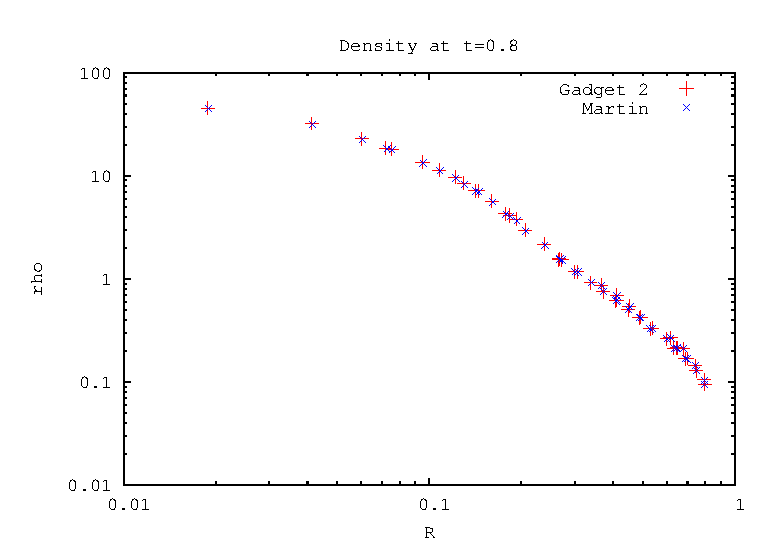
\includegraphics[width=\textwidth]{logrho0.8.eps}
%\caption{}
\end{figure}

\begin{figure}[H]
\centering
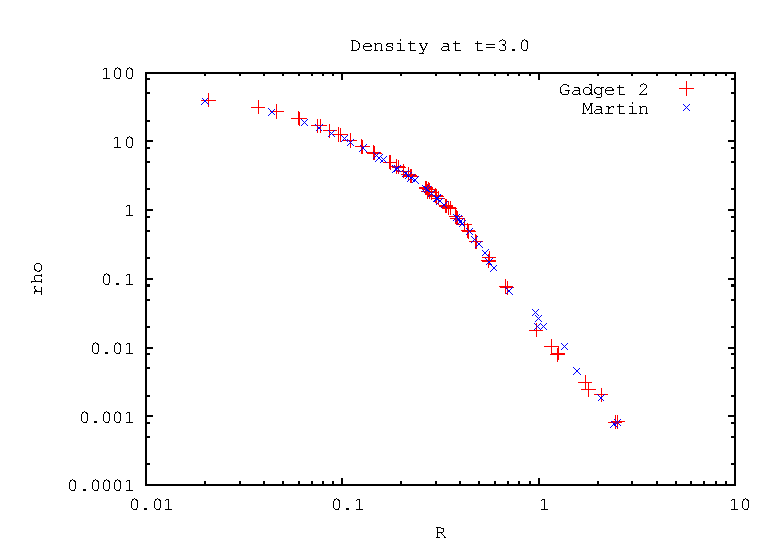
\includegraphics[width=\textwidth]{logrho3.0.eps}
%\caption{}
\end{figure}

\subsection*{Energy}
\begin{figure}[H]
\centering
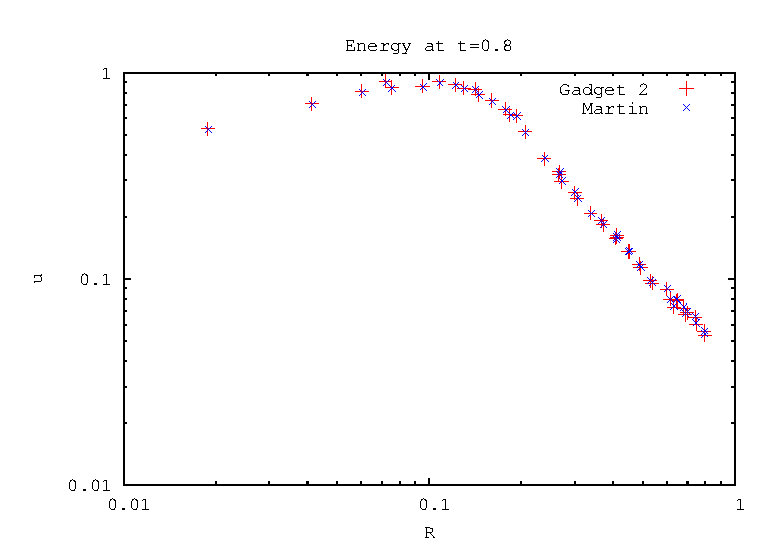
\includegraphics[width=\textwidth]{logu0.8.eps}
%\caption{}
\end{figure}

\begin{figure}[H]
\centering
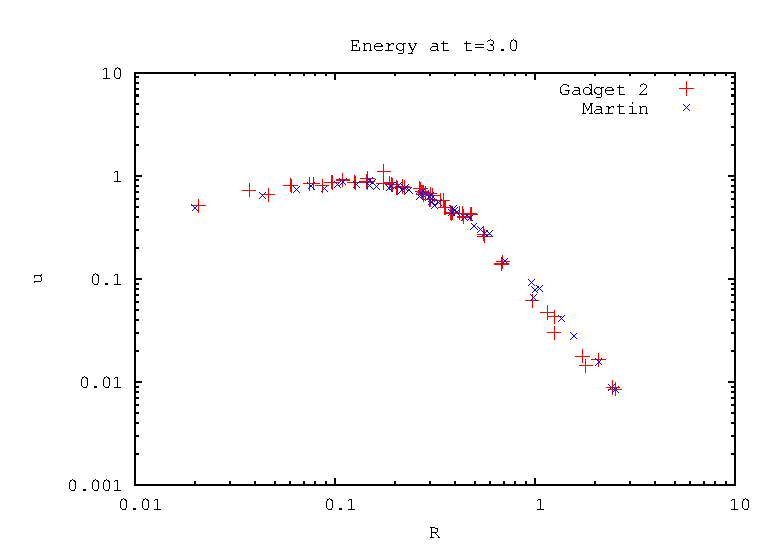
\includegraphics[width=\textwidth]{logu3.0.eps}
%\caption{}
\end{figure}

\subsection*{Entropy}
\begin{figure}[H]
\centering
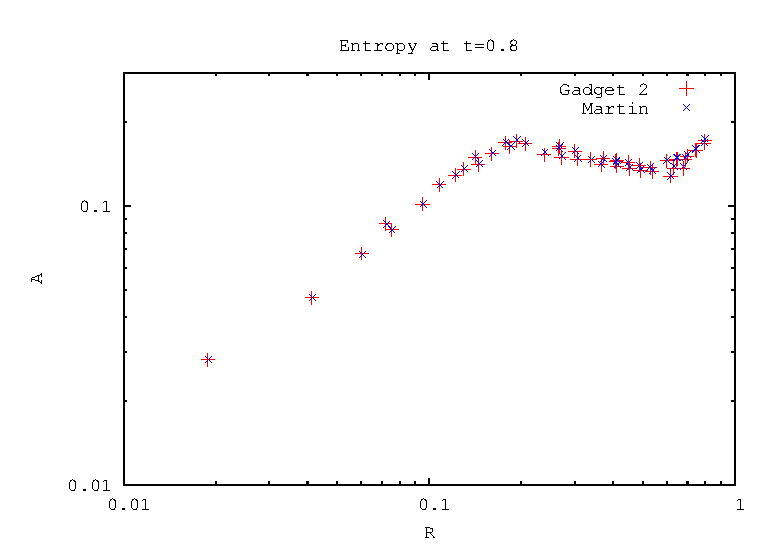
\includegraphics[width=\textwidth]{logA0.8.eps}
%\caption{}
\end{figure}

\begin{figure}[H]
\centering
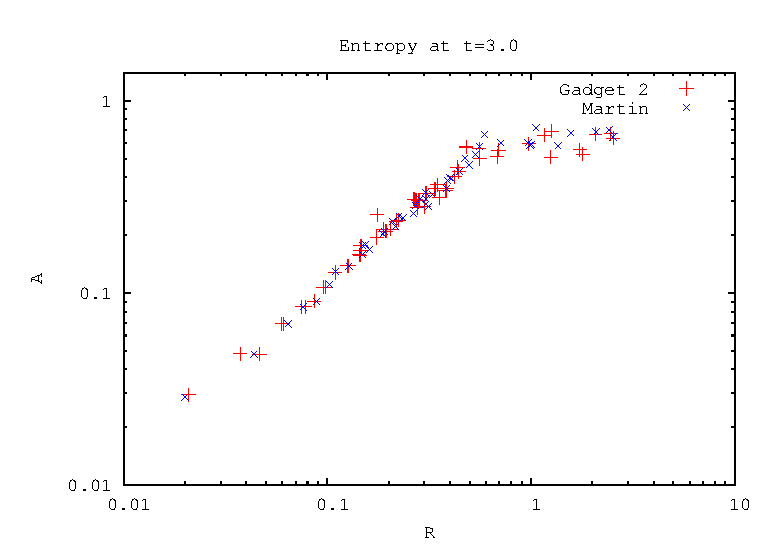
\includegraphics[width=\textwidth]{logA3.0.eps}
%\caption{}
\end{figure}


\label{lastpage}
\end{document}
